\section{Results}\label{results}

In this section, we describe our findings. Participants are referred to by pseudonyms \textit{P1--33}. P1--28 were included in our quantitative tests and results. P32--33 completed a variant of the study that involved use of a personal laptop. To convey representativeness of the findings, observations are accompanied with numbers indicating how many participants an observation reflects (e.g., ``(5)'' means 5 participants).

\subsection{Effect of FFL on task success}

Overall, there was significant improvement in task time, self-reported ease, and readability when participants used FFL for editing tasks (E1 \& 2), and no perceived difference for creation tasks (C1 \& 2).

\subsubsection{Completion rate} Overall, participants completed tasks at about the same rate when using FFL and LaTeX. Most participants succeeded in most tasks: altogether, participants reached the time limit on less than 20\% of tasks, amounting to 6 failed FFL tasks and 12 failed LaTeX tasks. The most difficult task for LaTeX seemed to be task E2 where 8 participants failed to complete in the LaTeX condition ($p=0.025$, {Fisher's Exact Test}~\cite{fisher}).
When asked to indicate the extent to which they were able to do what they wanted on a 7-point Likert scale (Figure \ref{fig:responses}), there was no significant difference between FFL and LaTeX ($F=0.792$, $p=0.565$).
A complete listing of per-task completion rates appears below in \hyperref[tab:count_fail_task]{Table~\ref{tab:count_fail_task}}.

\subsubsection{Speed}

\begin{figure}
    \centering
    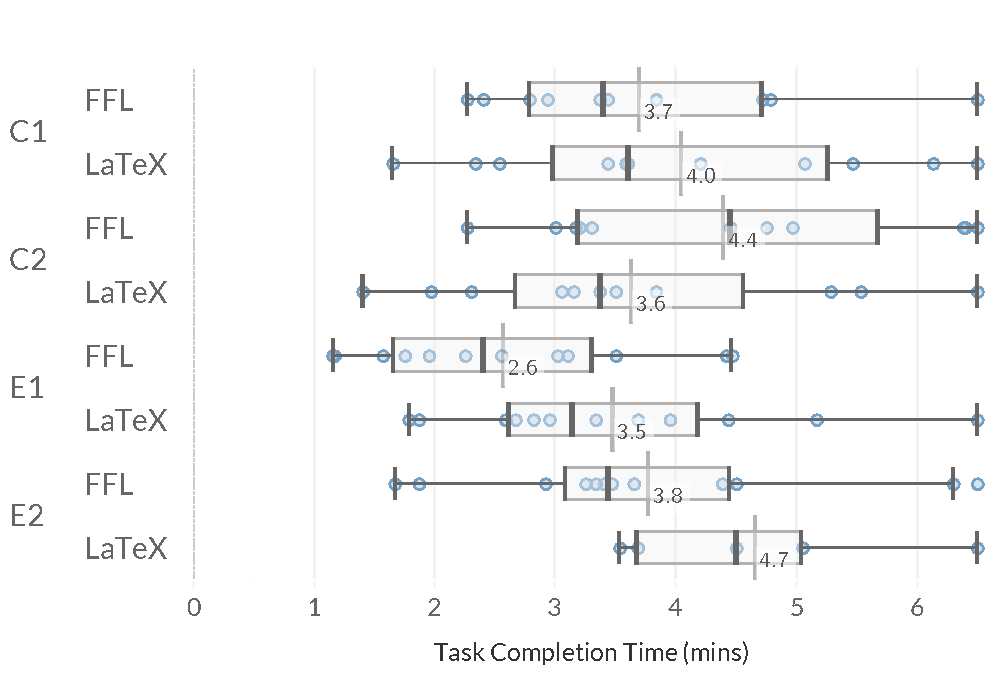
\includegraphics[width=\linewidth]{figures/Timing.pdf}
    \caption{Task completion time. Participants completed tasks E1 \& 2 significantly faster with FFL than with LaTeX. \normalfont Box-and-whiskers depict median, quartiles, and extrema (within 1.5 IQR). An additional, taller vertical line annotates the average. Individual times are rendered as dots in the background. Incompletes are encoded as maximum time. \zed{Per-row mean time and standard deviation appear in \hyperref[tab:speed_table]{Table \ref{tab:speed_table}}.}}
    \Description{Boxplot showing completion times by task and interface. The median completion time is lower with FFL than LaTeX for tasks C1, E1, and E2; and higher for task C2. Tasks C1 and C2 see greater variance in task completion time regardless of interface. For tasks E1 and E2, the median, average, minimum and maximum time are shorter with FFL than LaTeX.}
    \label{fig:timing}
\end{figure}

As depicted in \hyperref[fig:timing]{Figure~\ref{fig:timing}}, participants completed the complex editing tasks (E1 \& E2) more quickly with FFL than with LaTeX. A linear mixed-effects model found the interface to have a significant effect ($F=6.7$, $p=0.02$). Other significant effects include task ($F=11$, $p=2\times10^{-5}$) and task-interface interaction ($F=6.8$, $p=0.001$); task order was not significant. As implied by the task-interface interaction effect, the effect of FFL was stronger for some tasks than others. Fitting the same model to the pairs of creation (C1 \& 2) and editing (E1 \& 2) tasks separately, the effect of FFL was significant for editing tasks ($F = 27$, $p=7\times10^{-5}$), but not for the creation tasks ($p\approx1$). 
\zed{While we note that the test statistics are influenced by our choice to cut off participants at 6.5 minutes, a visual inspection suggests the above trends hold for participants who were not cut off: FFL decreased task time for the 0th--75th quartile participants, none of whom were cut off before completing the task (see Figure~\ref{fig:timing}). Our observations during the study revealed no clear signs that participants were further from completion when cut off in the FFL condition than in the baseline condition.}

\begin{figure}
    \centering
    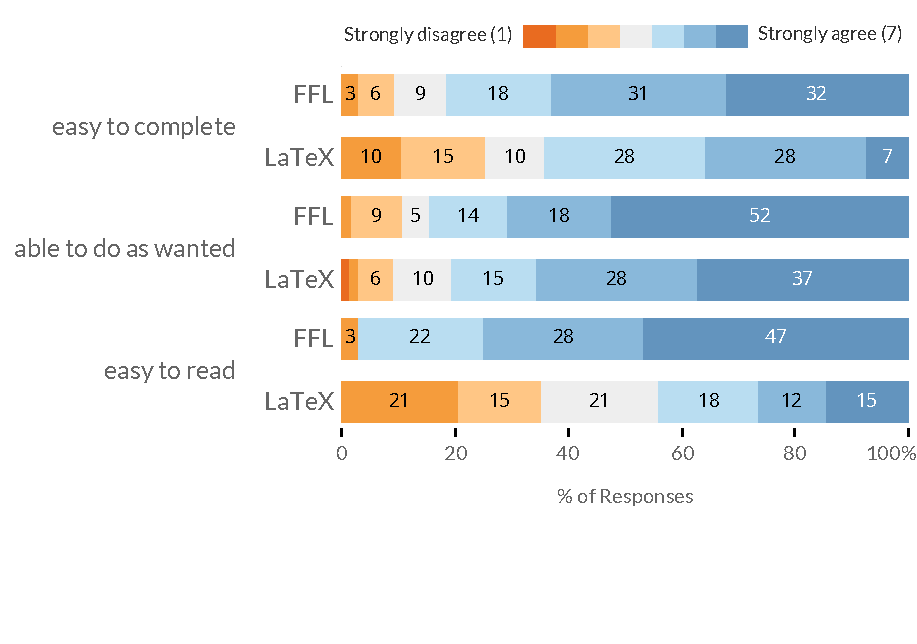
\includegraphics[width=\linewidth]{figures/Responses.pdf}
    \vspace{-2.5em}
    \caption{Self-reported ease for timed tasks. On the whole, participants reported greater ease with FFL than with LaTeX. \normalfont Data comes from responses when participants were asked to indicate agreement (from "strongly disagree" (1) to "strongly agree" (7)) with the statement in the left column of the bar chart. Numbers indicate percentages of total responses relative to the row. \zed{Per-row medians and arithmetic means appear in Tables \ref{tab:ease_table}--\ref{tab:ease_to_read_table}}.}
    \Description{Stacked bar chart of self-reported ease for timed tasks (on a 7-point Likert scale). The three dimensions of ease are “easy to complete”, “able to do as wanted” and “easy to read.” Greater ease is reported with FFL for all three; this difference is slight for “able to do as wanted” and pronounced for “easy to complete” and “easy to read.”}
    \label{fig:responses}
\end{figure}

\subsubsection{Ease}\label{sec:ease}

Participants reported significantly higher ease in completing tasks with FFL than with LaTeX ($F=16$, $p=6\times10^{-4}$). On a 7-point Likert scale, participants reported \zed{a median score of 7, versus 6} with LaTeX (Figure~\ref{fig:responses}). Models fit on subsets of tasks showed the difference in ease to be significant for editing tasks E1 \& 2 ($F=19$, $p=2\times10^{-4}$), but not tasks C1 \& 2 ($p\approx1$).

Additional questions on the questionnaire indicate aspects of FFL that might have led to greater ease. Following the editing tasks E1 \& 2, participants reported significantly greater ease in reading augmentation code (Figure~\ref{fig:responses}) in FFL than with LaTeX ($F=23$, $p=6\times10^{-5}$). In the retrospective questionnaire, participants compared the ease of using FFL to LaTeX for a variety of primitive augmentation operations (Figure~\ref{fig:eos1}), reporting greater ease with FFL for coloring parts of formulas ($W=7$, $p<0.002$, \zed{mdn. 5 vs. 4}), labeling parts of formulas ($W=0$, $p<0.002$, \zed{mdn. 5 vs. 4}), and applying the style to multiple parts of the formulas ($W=24$, $p<0.002$, \zed{mdn. 5 vs. 2}), on a 1--5 scale.

% \begin{center}
\begin{figure}
    \centering
    \vspace{-.5ex}
    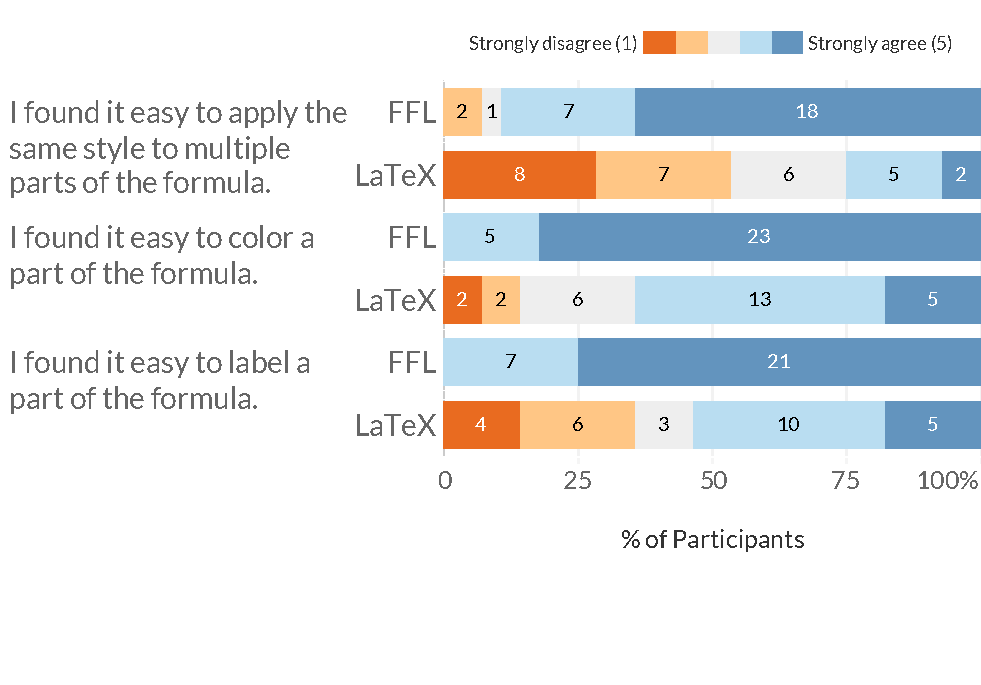
\includegraphics[width=\linewidth]{figures/EOS-1.pdf}
    \vspace{-2.5em}
    \caption{Ease-of-use ratings in retrospective questionnaire. \normalfont Ease was reported on three dimensions for both FFL and LaTeX (shown in the leftmost labels on the bar chart). % \normalfont Participants participants were asked to rate on a scale from "strongly disagree" (1) to "strongly agree" (5) on their agreement with the statement on the left after each task.
    \vspace{-1ex}}\Description{Stacked bar chart of ease-of-use responses in retrospective questionnaire, for three questions asked on a 5-point Likert Scale. The three questions are, “I found it easy to apply the same style to multiple parts of the formula,” “I found it easy to color a part of the formula,” and “I found it easy to label a part of the formula.” A majority of participants “strongly agreed” that FFL made tasks easy in these three ways. Agreement was weaker for LaTeX; with LaTeX, for applying the same style to multiple parts of the formula, 7 / 28 participants reported agreement (either a 4 or 5 out of 5); for coloring a part of the formula, 18 / 28; and for labeling a part of the formula 15 / 28.}
    \label{fig:eos1}
\end{figure}

\subsubsection{Differences in success}

While on the whole participants reported high levels of comfort with LaTeX in the introductory questionnaire, there was still considerable individual variation in comfort with both LaTeX and CSS. When we fit our model to take background factors into account,\footnote{When fitting a model with background factors as fixed effects, we remove the random effect of participant ID.} we observed years of experience of LaTeX as a significant predictor of task speed ($F=10$, $p=5\times10^{-5}$), with interface becoming insignificant ($F=5.4$, $p=.1$). For the creation tasks alone, years of experience with LaTeX is not significant  ($p=.3$). For the editing tasks, years of experience is significant ($F=10$, $p=3\times10^{-4}$), and interface remains a significant effect ($F=27$, $p=6\times10^{-5}$). Other background factors such as self-reported comfort with LaTeX or CSS were not significant predictors. Overall, additional years of experience of LaTeX reduced task completion times, though the trends vary considerably when broken down by task and interface pair.

\subsubsection{Interpretation}

In summary, participants completed tasks about as often with FFL and LaTeX. FFL led to quicker completion, with less difficulty. Post-hoc tests showed the effect to be significant for editing tasks E1 \& 2, but not creation tasks C1 \& 2. We explain this discrepancy with two observations. 

First, E1 \& 2 were performed after C1 \& 2. Some participants reported an initial learning curve with FFL, or encountered gaps or misconceptions regarding FFL during the first pair of tasks. These gaps and misconceptions were sometimes resolved by the time they began the second pair of tasks. Learning effects may provide a partial explanation: among 33 participants, our observation notes showed 23 participants making 35 critical mistakes \zed{(i.e., writing a spec that yielded compilation errors or incorrect outputs)} in C1 \& 2, reduced to 18 participants making 23 mistakes in E1 \& 2.
\zed{Gaps and misconceptions may have also been reduced when participants were given access to starter code in editing tasks E1\&2.}

Second, E1 \& 2 required participants to work with considerably more complex and denser markup along with some augmentation already integrated to begin with. E1 \& 2 reflect a setting where a formula has been augmented and the authors wish to experiment with alternative designs. We interpret this effect to indicate that FFL manifests more value as augmentation markup becomes larger; in the LaTeX baseline, this results in the markup languages becoming increasingly tangled and difficult to evolve, as discussed in greater detail in the next section.

\subsection{Effect of FFL on authoring experience}

In this section, we review observations, interviews, and questionnaire data to arrive at a comprehensive understanding of how FFL supports, and in some cases works against, the experience of formula augmentation. Overall, participants found FFL's ``core'' features useful (Figure~\ref{fig:features_use}). This section introduces strengths and shortcomings of FFL in terms of the cognitive dimensions of notation~\cite{ref:blackwell2003notational}, a framework used in programming language design to \zed{examine and discuss} the effect of language design choices.

\begin{figure}
    \centering
    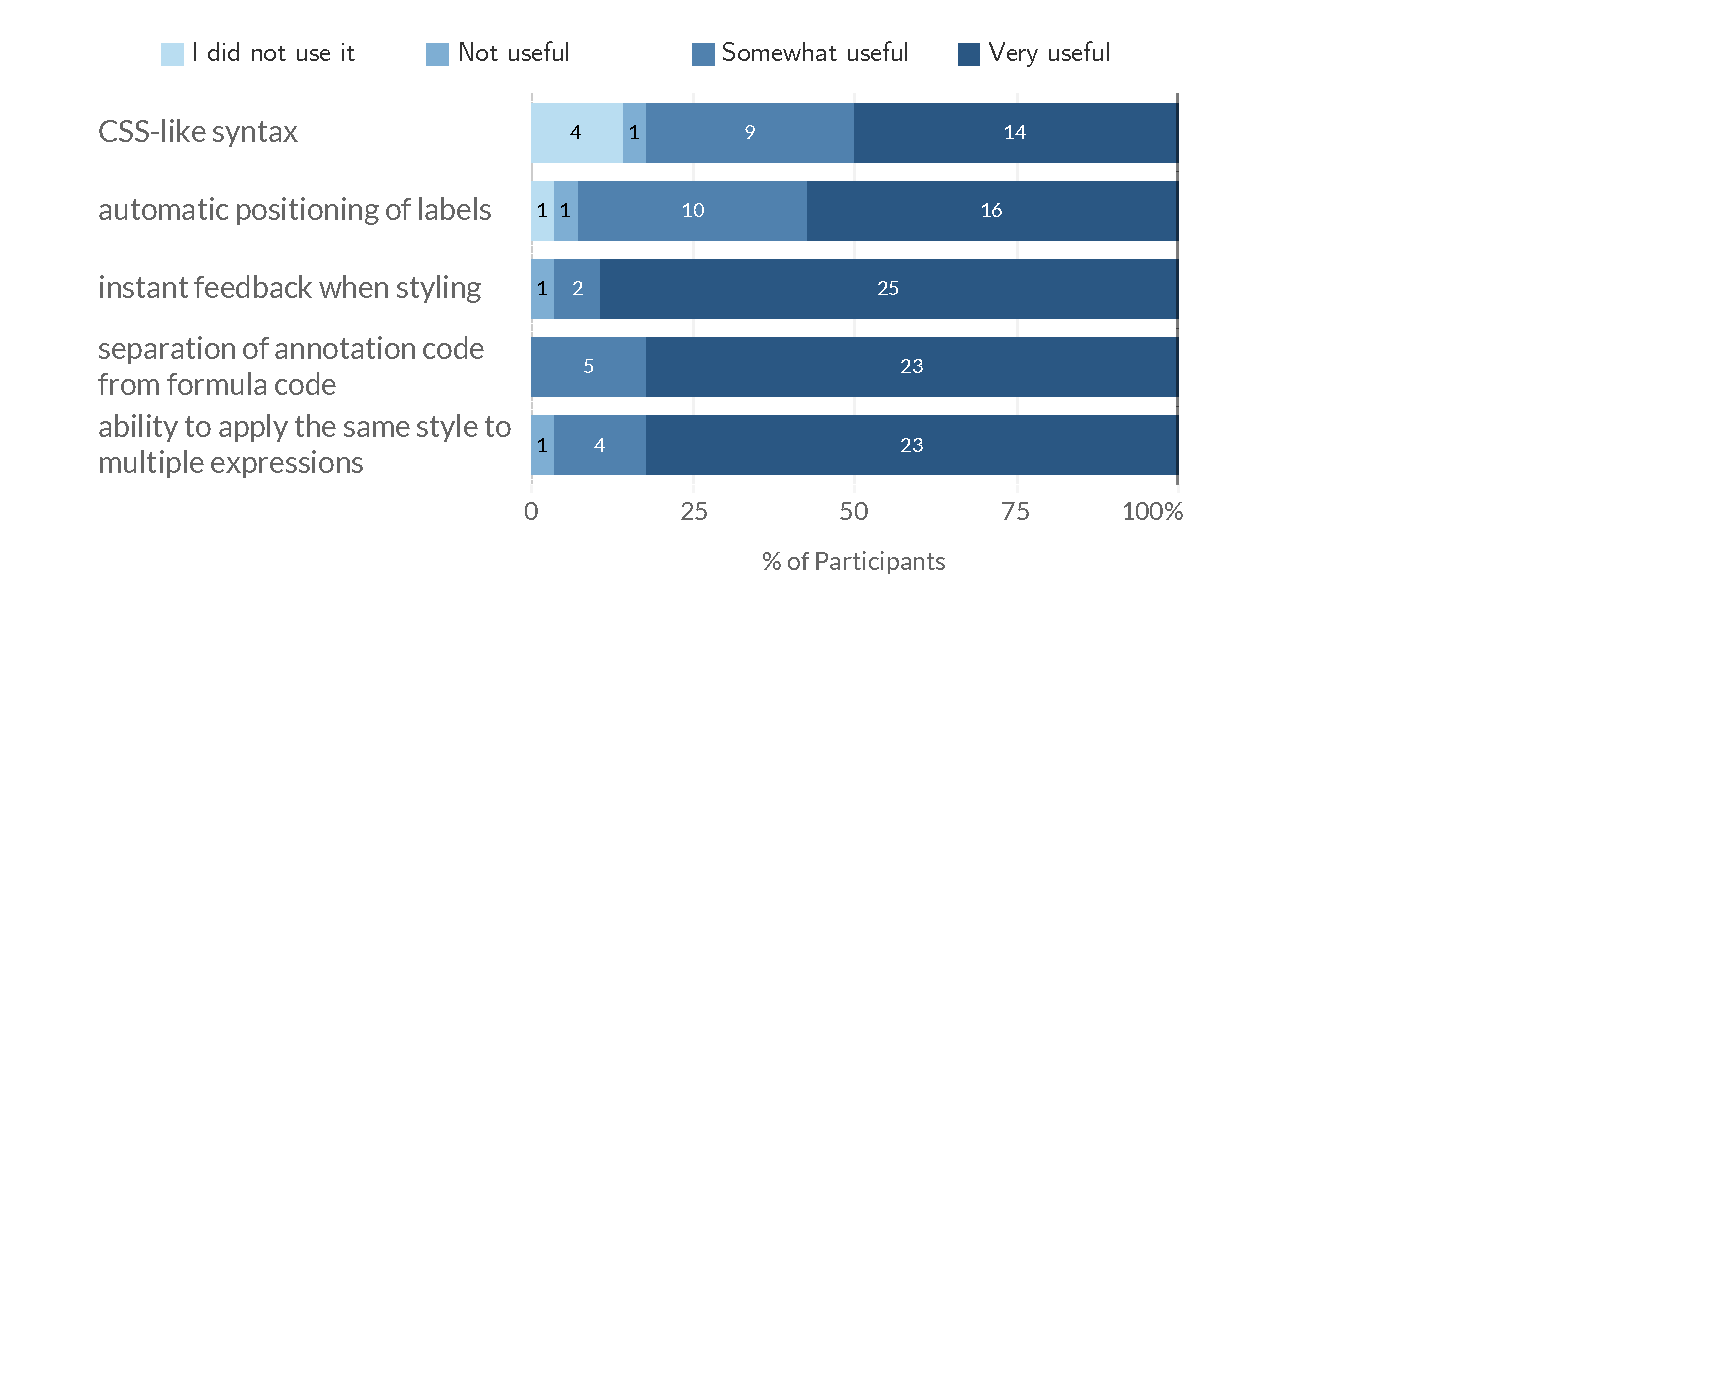
\includegraphics[width=\linewidth]{figures/Useful.pdf}
    \vspace{-3ex}
    \Description{Stacked bar chart of usefulness of 5 features (on a 4-point scale, including “I did not use it,” “not useful,” “somewhat useful,” and “very useful”). The five features are “CSS-like syntax,” “automatic positioning of labels,” “instant feedback when styling,” “separation of annotation code from formula code,” and “the ability to apply the same style to multiple expressions.” For all features except for “CSS-like syntax,” a majority of participants reported “very useful.” The vast majority of participants found “instant feedback,” “separation of annotation code from formula code,” and “the ability to apply the same style to multiple expressions” very useful. 14/28 participants found CSS-like syntax very useful, and 9/28 participants found it somewhat useful.}
    \caption{Usefulness of features. \normalfont Shown are participants' responses to the question ``How useful was \emph{[feature]} when you used FFL to augment math formulae?''
    }
    \label{fig:features_use}
\end{figure}

\subsubsection{Strengths} FFL improved the authoring experience as follows:

\paragraph{Viscosity}
FFL reduced the number of actions required to accomplish some goals. This was most clear when participants edited augmentations for multiple expressions at once. Participants frequently expressed appreciation for the ability to make cross-cutting changes with a single style specification (5), and wished for a similar capability for LaTeX (4). Making cross-cutting changes was described as more ``efficient'' (P4) and ``easier'' (P12, P24) with FFL. \zed{All but one} participant described the ability to apply one style to multiple expressions as very useful (Figure~\ref{fig:features_use}).

\paragraph{Hard mental operations}

FFL made it easier for participants to orient themselves to augmentation markup. LaTeX was the less preferred choice for reading markup (Figure~\ref{fig:responses}). LaTeX was described as difficult to read (16) and used complex or unintuitive syntax (6). The association of augmentations with expressions is difficult to understand due to the dependence on copious numbers of nested braces to associate them (14). Reading LaTeX was therefore described as ``holding a lot of moving pieces in my mind'' (P18), where ``it is a nightmare to look for what I am editing'' (P13). Reading challenges arose when participants had difficulty identifying expressions to which LaTeX commands applied (2), mapping from parts of the rendered formula to the corresponding LaTeX (5), reading and editing the markup (3), and pinpointing sources of errors (2).

In comparison, FFL seemed easier to read---we rarely heard similar criticisms levied against FFL. 16 participants explicitly mentioned their appreciation for the separation of formula markup from augmentation markup; this division was called a ``big advantage'' and ``very powerful'' (P13). The separation of annotation code from formula code was reported as ``very useful'' by the vast majority of participants in the retrospective questionnaire, and ``somewhat useful'' by all remaining participants. Participants rated the readability of FFL significantly higher than LaTeX (Section~\ref{sec:ease}).

\paragraph{Error proneness}

FFL removed a class of errors with its approach to associating expressions with augmentations. As mentioned in prior work~\cite{ref:head2022math}, one challenge of using LaTeX to augment formulas is to use braces correctly to associate augmentations with expressions. Participants described braces as ``annoying'' (P28), finding it difficult to find matching pairs of braces (6), and desiring the ability to find out which braces are redundant or missing (2). Braces were the most common kind of error we observed: at least some participants made a bracing error for each task (8 participants for task C1; 2 for C2; 6 for E1; and 8 for E2). Participants also encountered issues with using \texttt{\textbackslash{}def} correctly, writing arguments to commands in the right order, and other LaTeX compilation errors. As noted by participants, FFL did not see these difficulties due to its approach to associating augmentations with expressions (2).

\paragraph{Closeness of mapping}

In several situations, FFL provided a close mapping to the ways participants could envision expressing augmentations. Two participants described that the metaphor of CSS, including its use of selectors and attributes, was ``intuitive.'' The design of selectors allowed participants to indicate which expressions they wished to augment by selecting, and then copying and pasting, those expressions from the formula into their FFL specification (2). When asked to indicate the degree to which FFL ``did what I expected to,'' all but 2 participants agreed, and over half of the participants strongly agreed.

On the whole, participants developed comfort with a large number of primitives in a short amount of time. By the time they performed the exploratory authoring task, participants had developed enough comfort with the language that they frequently made use of color (24), labels with leader lines (19), and labels with extent markers (11). These augmentations made use of myriad language features, including single-character wildcards (15), sequence wildcards (15), unions (11), and the adjustment of label positions (9). See Appendix Section~\ref{sec: open_task_image} for examples.

\paragraph{Progressive evaluation}

The favorite feature of FFL was the instant feedback supported by the FFL runtime. More participants described this feature as ``very useful'' than any other feature. 7 participants explicitly indicated their appreciation for instant feedback. In contrast, the LaTeX toolset required slower compilation of the document to see the effect of one's changes to the markup (2), which was described as ``not very convenient'' (P21).

\subsubsection{Shortcomings}\label{sec:shortcomings} While FFL improved the experience of authoring formulas in numerous ways, it also introduced new challenges meriting new solutions to design and training:

\paragraph{Closeness of mapping}
FFL was not without a learning curve. Some participants found aspects of the CSS-like syntax challenging (8); this is in part because participants generally had low self-reported comfort with CSS (Section \ref{study-participants}). Participants also expressed discomfort with the \texttt{glob} syntax~\cite{UnixMan} for wildcards (1), and other aspects of LaTeX's math mode (5). These experiences serve as a reminder that FFL expects familiarity with CSS, glob, and LaTeX. We expect many authors seeking to use FFL in web documents would have this experience; though FFL still imposes a threshold to entry. An additional indicator of a learning curve is that 8 participants reviewed the cheat sheet before beginning their first task with FFL, suggesting that the tutorial was not enough to internalize the syntax. Similar challenges were observed for the LaTeX baseline, with participants forgetting commands taught in the tutorial (3) or failing to properly use commands from the cheat sheet (3).

While participants largely succeeded in selecting expressions with the selector syntax, several participants desired support for direct selection through mouse interaction with the formula (3). Similarly, participants desired the ability to highlight expressions corresponding to a selector (3). Participants also desired code generation (1) and no-code features (2), where style code could be partially or completely generated for the author. Direct selection features are beyond the scope of a language design, though they might serve as useful additions to an editing environment.

\paragraph{Error proneness}

FFL removed some classes of errors, though they introduced friction for others. The current runtime provides only very limited support for error tolerance, reporting, and recovery. 6 participants introduced typos and had difficulty understanding why their augmentation markup was not working as intended when they failed to notice those typos.
Some of these typos arose from challenges related to ``closeness of mapping''---several participants used incorrect delimiters that perhaps best reflected a lack of familiarity with the base CSS syntax. 3 participants wished that FFL continued to render live even when errors were present in the markup. For these reasons, participants desired numerous standard editor affordances that assist in reducing errors, including autocomplete (7), syntax highlighting (2), and templates (3).

\paragraph{Visibility}
Any sufficiently complex language contains constructs users are unaware of. We observed several such constructs for FFL that were either undiscoverable or poorly suited once discovered.

First, participants expressed confusion around scoping augmentations. The default behavior of the FFL runtime is to apply selectors globally across an entire document. What should an author do when they wish for their augmentation rules to apply to only a single expression, formula, or single passage? Several authors had this specific question (8). The current solutions in FFL are (1) the \texttt{intersect} command; (2) an \texttt{:nth} selector that selects an indexed occurrence; (3) creating an indexable group in the formula markup by adding brackets around it; (4) using style overriding (i.e., using one rule to style all expressions, and a second rule to revert it for some subset of those expressions). These features were largely unused, perhaps due to issues of discoverability or learnability. At least 2 participants expressed some confusion with overriding.

Second, participants desired more influence over the appearance of labels, including label size (4), color (3), and font-weight (3). While the \texttt{.ffl-label} class is applied to all labels for just this purpose, participants were not often aware of it. These undiscovered features represent opportunities to either increase visibility or redesign constructs to be easier to guess.

\paragraph{Expressiveness}
Expressiveness is not a cognitive dimension of notation, though we discuss it here as a catchall for controls participants desired that FFL did not provide. One often-desired feature was the ability to assign a single label to multiple expressions simultaneously. For example, in the exploratory task, participants often wanted to create one label for ``slope'' and connect it via leader lines to all four $\beta$ terms in the formula (9). The default behavior of FFL is to assign a label to only the first matched expression in a formula. As one participant noted, this made the behavior of FFL inconsistent, because style rules applied to all matching expressions, while labels applied to only the first matched expression (P23). Several participants wished for different behavior from the automatic label layout algorithm (4), and desired the ability to fine-tune label layout beyond FFL's current capabilities (3).
